% !TEX root = ../ausarbeitung.tex
%Erklärung des Nutzertests mit Testgruppe, was herausgefunden werden soll:
%A: Macht so ein Spiel für Partnerzahlen Spaß?
%B: Welche Version ist besser?
\chapter{Evaluation} %TODO Ref
Im Rahmen dieser Arbeit wird ein Nutzertest durchgeführt, um zwei Fragen zu beantworten. Zunächst soll überprüft werden, ob dieses Additionsspiel zur Unterstützung des Lernprozesses bei Addition über Partnerzahlen den Kindern Spaß bereitet. Außerdem soll ermittelt werden, welche der beiden implementierten Versionen besser bei den Kindern ankommt. Zur Beantwortung wird der GEQ Fragebogen zur KidsGEQ\cite{Poels2008b} Variante abgewandelt, damit Grundschüler alle Fragen verstehen und beantworten können.
\section{Game Experience Questionnaire}
Der Game Experience Questionaire wurde 2013 an der Universität für Technologie in Eindhoven definiert \cite{IJsselsteijn2013}.
Beim normalen GEQ werden 3 Module eingebaut:
\begin{itemize}
\item Core questionaire
\item Social Presence Module
\item Post-game Module
\end{itemize}
Diese Module werden direkt nach einer Spielrunde durchgegangen, dabei testen die ersten beiden Module, wie der Spieler sich beim Spielen gefühlt hat, während das Post-Game Module testet, wie der Spieler sich nach dem Beenden des spielens gefühlt hat. Da für meinen Nutzertest nur das erste Modul relevant ist, wird auf die genaue Erläuterung, der anderen beiden Module, verzichtet.
\subsection{Core questionaire}
In diesem Teil werden dem Spieler Fragen aus den Kategorien Challenge, Competence, Flow, Immersion, Negative Affect, Positive Affect und Tension gestellt, welche im Folgenden näher erläutert werden. Um eine gute Messung zu erzielen und Puffer zu haben, um wenn nötig Fragen streichen zu können, sollten fünf Fragen pro Kategorie verwendet werden. In der Auswertung muss hier außerdem die Gewichtung der Fragen überprüft werden, da es sein kann, dass bei der Ausführung, mit einer Frage Probleme auftreten können. Wenn sie zum Beispiel nicht verstanden wurde, kann es sein, dass diese Frage aus der Auswertung entfernen werden muss.
\subsubsection{Challenge}
Mit den Challenge Fragen wird beim GEQ der Schwierigkeitsgrad des Spiels ermittelt. Dieser kann durch mehrere Faktoren beeinflusst werden. Zum einen kann die Aufgabe einfach schwer gewählt sein, aber auch durch die technische Umsetzung und dem Design des Spiels, kann der Schwierigkeitsgrad angehoben werden. Auf diesen Einfluss wird in der Diskussion noch weiter eingegangen.\\
Eine beispielhafte Frage aus der Kategorie Challange wäre: \qq{Ich habe mich herausgefordert gefühlt}.
\subsubsection{Competence}
In der Competence Kategorie sollen Fragen beantwortet werden, die darauf abzielen, ob das Spiel intuitiv verständlich ist. Das heißt der Spieler sollte zu jeder Zeit wissen, was seine Aufgabe ist und wie er der Erfüllung dieser Aufgabe näher kommt.\\
Eine beispielhafte Frage aus der Kategorie Competence wäre: \qq{Ich war gut in dem Spiel}.
\subsubsection{Flow}
Der Flow-Wert beschreibt wie stark das Spiel die Aufmerksamkeit des Spielers eingenommen hat und wie 'vertieft'  er in das Spiel ist.\\
Eine beispielhafte Frage aus der Kategorie Flow wäre: \qq{Ich habe alles ummich herum vergessen}.
\subsubsection{Immersion}
In dieser Kategorie soll geprüft werden, wie die Ästhetik des Spiels ist. Dies betrifft sowohl, ob das Spiel visuell überzeugen kann, als auch, ob durch das Spiel die Fantasie des Spielers anregeregt werden kann.
\\
Eine beispielhafte Frage aus der Kategorie Immersion wäre: \qq{Ich fand das Spiel beeindruckend}.
\subsubsection{Positive Affect}
Unter dieser Kategorie versteht man Fragen, die ermitteln sollen, ob das Spiel positive Emotionen beim Spieler hervorrufen. Diese führen dazu, dass sich der Spieler durch das Spiel besser fühlt, da er zum Beispiel lachen musste.
\\
Eine beispielhafte Frage aus der Kategorie Positive Affect wäre: \qq{Das Spiel hat mich von Zeit zu Zeit zum Lachen gebracht}.
\subsubsection{Negative Affect}
Hier soll über Fragen ermittelt werden, ob das Spiel negative Emotionen beim Spieler hervorruft. Diese Emotionen können dazu führen, dass das Spiel dem Spieler keinen Spaß bereitet. Bei bestimmten Genres, wie Horrorspielen, können negative Emotionen, wie Angst, allerdings auch gewollt sein. Im Fall von MathSnake sollten diese aber möglichst minimiert werden.
\\
Eine beispielhafte Frage aus der Kategorie Negative Affect wäre: \qq{Ich habe mich gelangweilt}.
\subsubsection{Tension}
In dieser Kategorie zielen die Fragen auf die Gemütslage des Spielers ab. Hier können Erkenntnisse darüber gewonnen werden, ob das Spiel noch zu unausgereift ist. Dies ist dann der Fall, wenn der Spieler sich über das Spiel mehrfach beschwert, da er weiß, wie er sein Ziel erreichen kann, aber zum Beispiel die Steuerung zu sensibel oder verzögert ist.
\\
Eine beispielhafte Frage aus der Kategorie Tension wäre: \qq{Beim Spielen lief es nicht so, wie ich es wollte}.
\subsubsection{Bestimmung der Kategoriewerte}
Um den Wert jeder Kategorie für einen Teilnehmer des Nutzertests zu bestimmen, werden die Antwortmöglichkeiten von 0 bis 4 gewichtet. Anschließend werden alle Werte der jeweiligen Kategorie nach dieser Skala addiert und durch die Anzahl an Fragen geteilt. Es wird also der Mittelwert gebildet. 
\section{Umsetzung des KidsGEQ}
In der umgesetzten Version werden pro Kategorie drei Aussagen gewählt, die zunächst ins Deutsche übersetzt und anschließend in möglichst für Kinder leicht verständliche Sprache umformuliert werden. Diese 21 Aussagen sollen nun von den Kindern anhand einer Skala beantwortet werden. Diese Skala ist in fünf Kategorien aufgebaut: 'überhaupt nicht', 'ein wenig', 'mittel', 'ziemlich', 'sehr'. Die Frage an die Kinder ist, wie stark sie der jeweiligen Aussage zustimmen. Der Grad der Zustimmung wird zusätzlich durch einen Farbcode hervorgehoben, der in Abbildung \ref{fig:farbskala} dargestellt wird. 

\begin{figure}[htb]
	\centering
	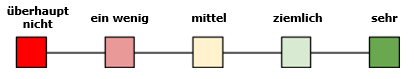
\includegraphics[width=0.75\textwidth]{farbskala}
	\caption{Farbskala der einzelnen Fragen\label{fig:farbskala}}
\end{figure}

Außerdem wurde eine weitere Frage zu den 21 Ankreuzfragen hinzugefügt, um abzufragen, wie gut die Kinder mit der Steuerung zurecht gekommen sind. Abschließend zu diesen 22 Ankreuzfragen gab es noch drei schriftliche Fragen um am Ende eine klare Antwort auf die Forschungsfragen zu erhalten.
\section{Durchführung des Nutzertests} %TODO Zufällige Version?
Der Nutzertest wurde mit fünf Grundschulkindern im Alter von 6 bis 10 Jahren (M= 8.4 , SD= 1.51) durchgeführt. Aufgrund der Stichprobengröße verzichte ich darauf, inferenzstatistische Verfahren anzuwenden und beschränke mich auf deskriptive Werte.\\
\\
Der Nutzertest wurde in zwei Phasen durchgeführt. Zunächst durften die Kinder eine Version für zehn Minuten spielen. Anschließend gab es den ersten Fragebogen mit den 22 Fragen. Es folgte eine kurze Pause von ca. fünf Minuten, in der sich das Kind mit etwas komplett anderem beschäftigt wurde, um zwischen beiden Versionen eine klare Trennung zu gewährleisten. Anschließend  spielte das Kind die zweite Version für weitere zehn Minuten. Nach dieser Spielzeit wurde ein weiterer KidsGEQ-Fragebogen in Verbindung mit drei abschließenden schriftlichen Fragen ausgefüllt. Insgesamt ergab dies eine Versuchsdauer von ca. 30 Minuten pro Person.


\hfil\rule{0.4\textwidth}{0.4pt}